\documentclass[10pt,a4paper]{article}
\usepackage{amsmath}
\usepackage{amsfonts}
\usepackage{amssymb}
\usepackage{natbib}
\usepackage{graphicx}
\usepackage[left=2cm,right=2cm,top=2cm,bottom=2cm]{geometry}
\usepackage{arydshln}

\title{Unbiased Noise Characterization for Geodetic Data}
\author{Trever T. Hines and Eric A. Hetland}
\begin{document}

\maketitle
\section{Introduction}\label{sec:Introduction}


The noise in geodetic data, which we consider to be any observed deformation that is not representative of the cohesive crustal block, is temporally correlated. It is necessary to accurately quantify this noise before the data is used to make geophysical inferences. A power-law relationship is often used to described the frequency content of noise in geodetic data \citep{Agnew1992}.  The power spectral density of power-law noise is described as 

\begin{equation}\label{eq.PowerLaw}
  P(f) = P_o f^{-n}
\end{equation}
where $f$ is frequency, $n$ is the spectral index and $P_o$ is the amplitude. Analysis of time series from strain and tilt meters \citep{Wyatt1982,Wyatt1989}, electronic distance measurements \citep{Langbein1997}, and short-baseline GPS \citep{King2009} indicates that temporally correlated noise can be attributed, at least in part, to an unstable geodetic monument. With the exception of \citet{King2009}, the referenced studies have found that localized motions of the monument can be modeled as a random walk process ($n=2$). GPS data, which is prone to additional non-physical sources of error \citep[e.g.][]{King2010}, has been described as a combination of white noise ($n=0$) and flicker noise ($n=1$) \citep{Zhang1997,Mao1999,Williams2004}. \citet{Langbein2008}, who used longer GPS timeseries,  found that GPS data in Southern California and Nevada contains white noise and some combination of flicker noise and random walk noise that varies between stations. It was suggested by \citet{Langbein2008} that random walk noise in GPS data can be attributed to monument instability while flicker noise can be attributed to non-physical errors introduced in deriving the displacement timeseries.  

No single noise model is universally appropriate for geodetic data, and the most rigorous of studies involving geodetic data should estimate a noise model for each station.  \citet{Langbein1997} introduce a maximum likelihood (ML) method for determining the optimal values for $P_o$ and $n$ (or the hyperparameters for any other assumed model). This method has become the standard technique for characterizing noise in geodetic data \citep{Langbein2004,Langbein2008,Zhang1997,Mao1999,Williams2004,King2009,Murray2017}.  

Recently, \citet{Langbein2012} demonstrated with synthetic data consisting of white and colored noise that the ML method is biased towards inferring a small component of colored noise in short timeseries.  The bias is appreciable when the length of the timeseries is less than or comparable to the cross-over period, which is the period at which the power of the colored noise exceeds the power of the white noise. \citet{Langbein2012} claims that the colored noise tends to be underestimated because it is indistinguishable in the power spectra of the data. We do not find this explanation to be satisfying. If the length of the timeseries is comparable to or less than the cross-over period then we would expect the estimated colored noise to have a high variance but this does not explain why there is a bias. In this paper we explain why the ML method from \citet{Langbein1997} is biased, and we demonstrate that an alternative approach, known as the restricted maximum likelihood (REML) method, does not suffer from this bias and has practically no additional computational burden. 

\section{Maximum likelihood methods}

Let $\mathbf{d_*}$ denote a column vector of $n$ observations. We treat $\mathbf{d_*}$ as a realization of the random vector

\begin{equation}\label{LangbeinModel}
  \mathbf{d} = \mathbf{Gm} + \mathbf{\epsilon},
\end{equation}
where $\mathbf{\epsilon}$ is the data noise vector, $\mathbf{G}$ is a $n \times m$ matrix with linearly independent columns that are used to describe geophysical signal in $\mathbf{d}$ (e.g. secular rates, coseismic offsets, postseismic transience, etc.), and $\mathbf{m}$ is a column vector of $m$ model parameters which have uninformative priors (i.e. $\mathbf{m} \sim \mathcal{N}(\mathbf{0},\lambda\mathbf{I})$ in the limit as $\lambda \to \infty$).  We assume that the data noise can be described as $\mathbf{\epsilon} \sim \mathcal{N}(\mathbf{0},\mathbf{\Sigma}(\mathbf{\theta}))$, where $\mathbf{\theta}$ are the hyperparameters which we want to find appropriate values for. Ideally, we would selects $\mathbf{\theta}$ such that the probability of drawing $\mathbf{d_*}$ from $\mathbf{d}$, $p_\mathbf{d}(\mathbf{d_*}|\mathbf{\theta})$, is maximized. However, the uninformed prior on $\mathbf{m}$ makes $\mathbf{d}$ improper and $p_\mathbf{d}$ is zero for all choices of $\mathbf{\theta}$. We must instead seek an alternative likelihood function to maximize. 

The ML method from \citet{Langbein1997} chooses $\mathbf{\theta}$ such that the probability of sampling the least squares residual vector,

\begin{equation}\label{ResidualRealization}
  \mathbf{r}_* =  \left(\mathbf{I} - \mathbf{G}\left(\mathbf{G}^T\mathbf{\Sigma}^{-1}\mathbf{G}\right)^{-1}\mathbf{G}^T\mathbf{\Sigma}^{-1}\right)\mathbf{d_*},
\end{equation}  
from $\mathbf{\epsilon}$ is maximized. To put it explicitly, The ML method maximizes the probability density function

\begin{equation}\label{MLProb}
p_\mathbf{\epsilon}(\mathbf{r}_*|\mathbf{\theta}) = 
\left(\frac{1}{(2\pi)^n\left| \mathbf{\Sigma}(\mathbf{\theta}) \right|}\right)^{\frac{1}{2}} 
e^{-\tfrac{1}{2}\mathbf{d}_*^T\mathbf{K(\mathbf{\theta}})\mathbf{d}_*}
\end{equation}
with respect to $\mathbf{\theta}$, where
\begin{equation}
\mathbf{K} = \mathbf{\Sigma}(\mathbf{\theta})^{-1} - 
             \mathbf{\Sigma}(\mathbf{\theta})^{-1}\mathbf{G}
             \left(\mathbf{G}^T\mathbf{\Sigma}(\mathbf{\theta})^{-1}\mathbf{G}\right)^{-1}
             \mathbf{G}^T\mathbf{\Sigma}(\mathbf{\theta})^{-1}.
\end{equation}
Implementations of the ML method typically maximize the logarithm of eq. (\ref{MLProb}) with the downhill simplex method \citep{Press2007}. It is important to recognize that the ML method assumes that $\mathbf{r}_*$ is a representative sample of $\mathbf{\epsilon}$. This assumption is only valid when $n$ is sufficiently large. To elaborate, we note that $\mathbf{r_*}$ is a sample of the random variable

\begin{equation}\label{ResidualVariable}
  \mathbf{r} =  \left(\mathbf{I} - \mathbf{G}\left(\mathbf{G}^T\mathbf{\Sigma}^{-1}\mathbf{G}\right)^{-1}\mathbf{G}^T\mathbf{\Sigma}^{-1}\right)\mathbf{d},
\end{equation}  
which is distributed as
\begin{equation}\label{ResidualDistribution}
  \mathbf{r} \sim \mathcal{N}\left(\mathbf{0},\mathbf{\Sigma} - \mathbf{G}\left(\mathbf{G}^T\mathbf{\Sigma}^{-1}\mathbf{G}\right)^{-1}\mathbf{G}^T\right).
\end{equation}
The term being subtracted in eq. (\ref{ResidualDistribution}) is the covariance of the least squares prediction vector, which will typically get smaller as $n$ increases. The distribution of $\mathbf{r}$ will then tend towards that of $\mathbf{\epsilon}$ as $n$ increases. Thus we can only assume that $\mathbf{r}_*$ is a representative sample of $\mathbf{\epsilon}$ when $n$ is sufficiently large. We can also observe from eq. (\ref{ResidualDistribution}) that the variance of $\mathbf{r}$ will always be less than the variance of $\mathbf{\epsilon}$.  We believe this is the reason why the ML method from \citet{Langbein1997} is biased towards underestimating the noise in short timeseries.

Having demonstrated that the ML method from \citet{Langbein1997} is biased, we move on to discuss the restricted maximum likelihood (REML) method for selecting $\mathbf{\theta}$.  The REML method was introduced by \citet{Patterson1971}, and is now established in the Kriging community as an unbiased method for estimating covariance functions \citep[e.g.][]{Cressie1992}. The REML method can be understood by first considering a $(n-m)\times n$ matrix $\mathbf{R}$ which satisfies $\mathbf{R}\mathbf{G}=\mathbf{0}$.  We then consider the random variable $\mathbf{x}=\mathbf{R}\mathbf{d}$, which can be interpreted as the mapping of $\mathbf{d}$ onto a subspace that is orthogonal to the columns of $\mathbf{G}$. As opposed to $\mathbf{d}$, $\mathbf{x}$ is a proper random variable since it is independent of the prior on $\mathbf{m}$. The REML method chooses $\mathbf{\theta}$ such that the probability of drawing $\mathbf{x}_*=\mathbf{R}\mathbf{d}_*$ from $\mathbf{x}$, $p_\mathbf{x}(\mathbf{x}_*|\mathbf{\theta})$, is maximized. As noted by \citet{Harville1974}, the particular choice for $\mathbf{R}$ does not matter because it will only change the likelihood function which we are maximizing by a scale factor. Following \citet{Harville1974}, we let $\mathbf{R}$ have the properties $\mathbf{R}^T\mathbf{R} = \mathbf{I} - \mathbf{G}(\mathbf{G}^T\mathbf{G})^{-1}\mathbf{G}^T$ and $\mathbf{R}\mathbf{R}^T = \mathbf{I}$. The probability density function for $\mathbf{x}$ can then be written as 

\begin{equation}\label{REMLProb}
p_\mathbf{x}(\mathbf{x}_*|\mathbf{\theta}) =
\left(\frac{\left|\mathbf{G}^T\mathbf{G}\right|}
           {(2\pi)^{n-m}
            \left| \mathbf{\Sigma}(\mathbf{\theta}) \right| 
            \left| \mathbf{G}^T\mathbf{\Sigma}(\mathbf{\theta})^{-1}\mathbf{G} \right|}\right)^{\frac{1}{2}} 
e^{-\tfrac{1}{2}\mathbf{d}_*^T\mathbf{K}(\mathbf{\theta})\mathbf{d}_*} .
\end{equation}
Note the similarity between eq. (\ref{REMLProb}) and eq. (\ref{MLProb}). If programmed efficiently (see Appendix A) and if $m \ll n$, the computational cost of the REML method is practically equivalent to that of the ML method from \citet{Langbein1997}. What remains to be determined is whether the REML method remediates the bias in the ML method. We demonstrate that this is indeed the case with a numerical test. 

\section{Synthetic demonstration}
We compare the REML method and the ML method from \citet{Langbein1997} by using the two methods to estimate hyperparameters from snythetic data. This demonstration is modeled after the demonstration from \citet{Langbein2012} which highlights bias in the ML method. Our synthetic noise is a combination of white and random walk noise, which has a power spectral density described by

\begin{equation}\label{SyntheticFreq}
P(f) = \frac{\sigma_{rw}^2}{2\pi^2 f^2} + 2\sigma_w^2\Delta t,
\end{equation}  
where $\sigma_{rw}$ and $\sigma_w$ are hyperparameters for the random walk and white noise components, respectively. $\Delta t$ is the sampling period, which is set at one day. The cross-over frequency for the synthetic noise noise is then
\begin{equation}\label{Crossover}
f_o = \frac{1}{2\pi\sqrt{\Delta t}}\frac{\sigma_{rw}}{\sigma_w}.  
\end{equation}
In order to use the ML or REML method, we must express the power-law relationship in the frequency domain as a covariance matrix in the time domain. A general procedure for doing  so can be found in \citet{Langbein2004}. The components of the covariance matrix corresponding to eq. (\ref{SyntheticFreq}) can be concisely written as

\begin{equation}\label{Covariance}
\Sigma_{ij} = \sigma_{rw}^2 \min(i\Delta t,j\Delta t) + \sigma_w^2 \delta_{ij},
\end{equation} 
where $\delta_{ij}$ is the Kronecker delta function. Similar to \citet{Langbein2012}, we set $\sigma_{rw} = 1.3$ mm/yr$^{0.5}$ and $\sigma_w = 1.1$ mm. We generate 5,000 synthetic noise timeseries, which each have a length of 2.5 yr. 

We consider $\sigma_w$ to be known, for the sake of simplicity, and we want to estimate $\sigma_{rw}$ from the synthetic data. Although our synthetic data just consists of noise, we assume that the unknown underlying geophysical signal (i.e. $\mathbf{G}\mathbf{m}$) consists of a constant and linear trend. We estimates $\sigma_{rw}$ with the ML and REML methods using varying lengths of the synthetic timeseries. The timeseries lengths range from 0.1 yr to 2.5 yr at 0.1 yr increments. The distribution of estimated $\sigma_{rw}$ is shown in Figure \ref{fig:EstimateRW}. 

\begin{figure}
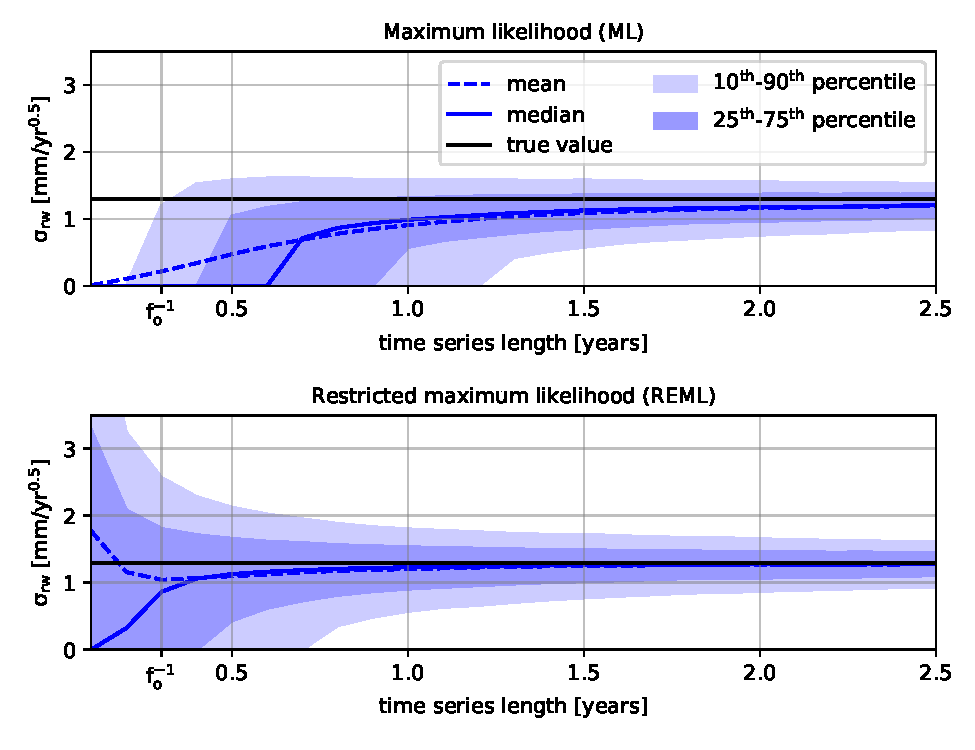
\includegraphics[scale=1.0]{figure_1.pdf}
\caption{Comparison of ML and REML method over varying lengths of the synthetic timeseries. The black line indicates the true random walk scale ($\sigma_{rw}=1.3$), the light blue region shows the 10-90 percentile of estimates, the dark blue region shows the 25-75 percentile of estimates, the solid blue line indicates the median, and the dashed blue line indicates the mean. Note that $f_o^{-1} \approx 0.3$.}   
\label{fig:EstimateRW}
\end{figure}

The distribution of $\sigma_{rw}$ estimated by the ML method indicates that there is a bias towards underestimating $\sigma_{rw}$ when the length of the timeseries is comparable to $f_o^{-1}$, which is 0.3 yr in this demonstration. The bias is appreciable when the timeseries is shorter than ${\sim}1$ yr, and estimates of $\sigma_{rw}$ cluster around 0.0 when the timeseries is shorter than $f_o^{-1}$. The distribution tightens up around the true value and remains relatively constant for timeseries with length greater than ${\sim}1$ yr. This is consistent \citet{Langbein1997} who said that the timeseries should be at least 5 times greater than $f_o^{-1}$ to get a good estimate of the random walk component. However, the mean and median of the distribution tends to be slightly less than the true value even when the full length of the timeseries is used.

In contrast, the REML method does significantly better at estimating $\sigma_{rw}$. For every timeseries length considered, the true value for $\sigma_{rw}$ is within the 25-75 percentile of estimated $\sigma_{rw}$. For timeseries longer than $f_o^{-1}$, the mean and median of estimated $\sigma_{rw}$ closely resembles the true value, indicating that the REML method is indeed unbiased. When the length of the timeseries is less than $f_o^{-1}$, the meand and median deviate from the true value and the variance of estimated $\sigma_{rw}$ sharply increases. For such short timeseries, the random walk component cannot be resolved because it is being masked by the white noise. 
  
\section{Discussion and conclusion}
We have demonstrated that the restricted maximum likelihood (REML) method for characterizing noise does not suffer from the bias inherent in the maximum likelihood (ML) method from \citet{Langbein1997}. Furthermore, the ML and REML methods have practically equivalent computational costs. We therefore argue that there is no reason to prefer the ML method over the REML method. Despite the fact that the REML method has been well estabished in the Kriging community and elsewhere \citep[e.g.][]{Wahba1985}, it does not seem to be appreciated in the geodetic community.  It is our intention to bring the REML method to light. We believe this is particularly necessary because the ML method has been frequently used in research and has been used in deriving public data products \citep[e.g.][]{Murray2017}. 

We also emphasize that the REML method is able to accurately characterize colored noise in timeseries that are shorter than what is required for the ML method. \citet{Langbein1997} and \citet{Langbein2012} have suggested that the length of a timeseries must be at least 5 to 10 times $f_o^{-1}$ in order to accurately characterize colored noise. Based on our synthetic demonstration, the REML method remains accurate for time series as short as $f_o^{-1}$.      

\section{Appendix}
(pseudo-code for REML)

\bibliographystyle{apalike}
\bibliography{mybib}  

\end{document}